\documentclass[ngerman]{beamer}

\usepackage{graphicx}
  \graphicspath{{images/}}
\usepackage[utf8]{inputenc}
\usepackage[T1]{fontenc}
\usepackage[ngerman]{babel}
\usepackage{amsmath}
\usepackage{hyperref}
\usepackage{lmodern}

% Default fixed font does not support bold face
\DeclareFixedFont{\ttb}{T1}{lmss}{b}{n}{11} % for bold
\DeclareFixedFont{\ttm}{T1}{lmss}{m}{n}{11}  % for normal
\DeclareFixedFont{\tts}{T1}{lmss}{lc}{n}{11}  % for normal

% Custom colors
\usepackage{color}
\definecolor{deepblue}{rgb}{0,0,0.6}
\definecolor{deepred}{rgb}{0.8,0,0}
\definecolor{deepgreen}{rgb}{0,0.7,0}
\definecolor{commentgrey}{rgb}{0.3,0.3,0.3}
\definecolor{deeporange}{RGB}{255,140,0}
\usepackage{listings,caption}

% Python style for highlighting
\newcommand\pythonstyle{\lstset{
		language=Python,
		captionpos=b,
		moredelim=[is][\ttb\color{deeporange}]{§}{§},
		basicstyle=\ttm,
		otherkeywords={self, yield, with},             % Add keywords here
		keywordstyle=\ttb\color{deepblue},
		morekeywords = [2]{MyClass,__init__,__iter__,__next__,__eq__,__gt__},         
		keywordstyle = [2]\ttb\color{deepred},
		moredelim=[is][\tts\color{orange}]{°}{°},
		moredelim=[is][\ttm]{!}{!},
		moredelim=[is][\ttb\color{deepblue}]{³}{³},
		stringstyle=\color{deepgreen},
		commentstyle = \color{commentgrey}\itshape,
		columns=flexible,
		numbers=left,
		tabsize=4,
		frame=,                         % Any extra options here
		showstringspaces=false            % 
}}


% Python environment
\lstnewenvironment{python}[1][]
{
	\pythonstyle
	\lstset{#1}
}
{}

\renewcommand{\lstlistingname}{Code}

\theoremstyle{definition}
\newtheorem{syntax}{Syntax}
\newtheorem{grammatik}{Grammatik}

\usetheme{Singapore}
\usecolortheme{rose}
\usefonttheme{professionalfonts}
\usepackage{appendixnumberbeamer}


\addtobeamertemplate{navigation symbols}{}{
	\ifnum\insertframenumber>\inserttotalframenumber%
	\relax
	\else%
	\usebeamerfont{footline}%
	\usebeamercolor[fg]{footline}%
	\hspace{1em}%
	\insertframenumber/\inserttotalframenumber
	\fi%
}

\title{Fortgeschrittenes Python}

\subtitle{Lamdba-Ausdrücke, Listcomprehension, Generatoren und Dekorateure}

\author{Jan Digeser}

\date{Programmierung in Python, 30.05.2018}

\subject{Fortgeschrittenes Python}

%\AtBeginSection[]
%{
%  \begin{frame}<beamer>{Inhalt}
%    \tableofcontents[currentsection]
%  \end{frame}
%}


\begin{document}

\begin{frame}
  \titlepage
\end{frame}

\begin{frame}{Inhalt}
  \tableofcontents
\end{frame}
\section{Einstieg}
\begin{frame}[fragile,allowframebreaks]{Vererbung und abstrakte Klassen}
	\begin{itemize}
		\item {Subklassen erben Methoden und Variablen}
		\item {Methoden können überschrieben werden}
		\item {\emph{isinstance(i,A)} ist \emph{True} wenn i Instanz von A oder
		einer Subklasse von A}
		\item {Mehrfachvererbung wird unterstützt}
	\end{itemize}
	\framebreak
	\begin{example}[Vererbung]
		\begin{python}
class Vogel:
	def fly(self):
		print("Flap Flap Flap")
		
class Geier(Vogel):
	aasfresser = True
	
class Pinguin(Vogel):
	def fly(self):
		raise NotImplementedError("Kann nicht fliegen")

		\end{python}		
	\end{example}

	\framebreak
	
	\begin{itemize}
		\item {Abstrakte Klassen erben von \emph{abc.ABC}}
		\item {Alle Methoden die mit \emph{@abstractmethod} dekoriert sind müssen implementiert werden}
	\end{itemize}
	\begin{example}[Abstrakte Klassen]
		\begin{python}
from abc import ABC, ABCMeta, abstractmethod

class MyABC(ABC): # class MyABC(metaclass=ABCMeta)
	
	§@abstractmethod§
	def test(self): °...°
	
		\end{python}		
	\end{example}
\end{frame}
\begin{frame}[fragile, allowframebreaks]{Iteratoren und Iterable}
	\begin{itemize}
		\item {\textbf{Iteratoren} liefern ein Element, jedes mal wenn man sie danach fragt (mit \emph{next()} )}
		\item {\textbf{Iterable} sind Objekte, von denen man einen Iterator erstellen kann (mit \emph{iter()} )}
		\item {(Fast) alle Container sind \emph{iterable}}
		\item {Sehr viele Funktionen benötigen \emph{Iterables} als Eingabe}
		\item {Wenn ein Iterator erschöpft ist, raised er \emph{StopIteration} beim Versuch das nächste Element zu holen}
		\end{itemize}
\framebreak
	\begin{figure}
		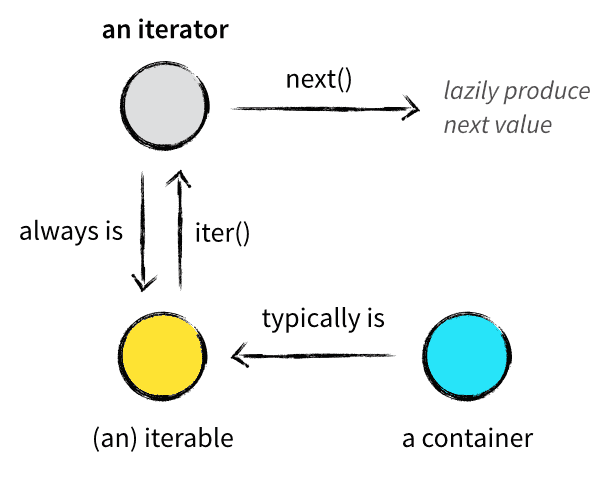
\includegraphics[scale=0.6]{relationships1.png}\break
		{\tiny Quelle: \url{http://nvie.com/img/relationships.png}}
	\end{figure}
\framebreak
\begin{exampleblock}
~
\begin{python}
class Iterable(ABC):
	
	§@abstractmethod§
	def __iter__(self) -> Iterator : ...
	
	
class Iterator(ABC):

	def __iter__(self) -> Iterator :
		return self

	§@abstractmethod§
	def __next__(self) -> object : ...
	
\end{python}
\end{exampleblock}
\end{frame}

\section{Lambda-Ausdrücke}

\begin{frame}[fragile]{Was sind Lambda-Ausdrücke?}
  \begin{itemize}
  \item {
    Anonyme (unbenannte) Funktionen
  }
  \item {
    Stammen aus dem \alert{Lambda-Kalkül} von Alonzo Church (1936)
  }
  \item {
  	Bilden Grundlage für funktionale Programmierung  
  }
  
  \end{itemize}
  \begin{syntax}
  	\begin{python}[numbers=none]
		lambda [parameter] : ausdruck
  	\end{python}
  \end{syntax}
\end{frame}

\begin{frame}[fragile,allowframebreaks]{Gebrauch von Lambda-Ausrücken}
	\begin{example}[Als normale Funktion]
		\begin{python}[numbers=none]
°>>>° quadriere = lambda x : x * x
°>>>° quadriere
<function <!lambda!> at 0x053F3D20>
°>>>° quadriere(3)
9
		\end{python}
	\end{example}
\end{frame}
\begin{frame}[fragile, allowframebreaks]{Map, Filter \& Reduce}
	\begin{itemize}
		\item {\textbf{map(f, iterable, ...)} wendet eine Funktion \emph{f} auf die Elemente von einer oder mehreren \emph{iterable} an}
		\item {\textbf{filter(f, iterable)} konstruiert einen Iterator mit den Elementen aus \emph{iterable}, für die \emph{f} wahr ist}
		\item {\textbf{itertools.reduce(f, iterable[, init])} wendet \emph{f} auf die ersten beiden Elemente von \emph{iterable} an und ersetzt diese, bis nur ein Wert übrig bleibt}
	\end{itemize}
	\framebreak
	\begin{example}[map, filter, reduce]
		\begin{python}[numbers=none]
°>>>° list( map( lambda x: x*2, [1, 2, 3, 4, 5, 6]))
[2, 4, 6, 8, 10, 12]
°>>>° list( filter( lambda x : x%3 == 1, [1, 2, 3, 4, 5, 6]))
[1, 4]
°>>>° list( reduce( lambda a, b: [*a, a[-1]+b], [10, 5, -3], [0]))
[0, 10, 15, 12]
		\end{python}
	\end{example}


\end{frame}

\section{Listenabstraktion}

\begin{frame}[fragile, allowframebreaks]{Erzeugen von Containern}
\begin{itemize}
	\item {Map, Filter und Reduce sind nicht ideal um einfache Container zu schaffen}
	\item {Reduce wurde mit Python 3 nach functools verbannt}
	\item {Comprehensions sind intuitiver, einfacher zu lesen und sehr effizient}
\end{itemize}
\begin{grammatik}
	\begin{python}[numbers=none]
		comprehension  = ausdruck comp_for
		comp_for 	   = "for" var "in" smth [comp_iter]
		comp_iter	   = comp_for | comp_if
		comp_if		   = "if" condition [comp_iter]
	\end{python}
\end{grammatik}
\framebreak[2]
\begin{itemize}
	\item {Comprehensions sind mit Listen, Mengen und Dictionaries möglich}
	\item {Man benutzt dabei eckige Klammern für Listen und geschweifte Klammern für Mengen und Dictionaries}
\end{itemize}
\begin{example}[einfache Comprehensions]
\begin{python}[numbers=none]
°>>>° [ x*x for x in [1,2,3,4,5] ]
[1, 4, 9, 16, 25]
°>>>° { x for x in range(7) if x % 3 == 1 }
{1, 4}
°>>>° { a: len(a) for a in ['aaa', 'a', 'abcd'] }
{'aaa': 3, 'a': 1, 'abcd': 4}
\end{python}
\end{example}
\framebreak
\begin{example}
	\begin{python}
°"""
Sei array ein 2D-Array zum Beispiel ein Spielfeld
Oft benoetigt man die Nachbarn einer Zelle 
(z.B. Minesweeper, Game of Life)
pos_x, pos_y ist die Position dieser Zelle
"""°

neighbors = [array[pos_x + xoff][pos_y + yoff] 
			 	for xoff in {-1,0,1}
				for yoff in {-1,0,1}
				if not xoff == yoff == 0
			]
	\end{python}
\end{example}
\end{frame}

\section{Generatoren}

\begin{frame}[fragile]{Wie schreibe ich einfacher Iteratoren?}
	\begin{itemize}
		\item Warum?
		\begin{itemize}
			\item {Klassen sind nicht schön}
			\item {Man muss eine bestimmte Form befolgen, die Platz verbraucht}
		\end{itemize}
	\end{itemize}
	\begin{figure}
		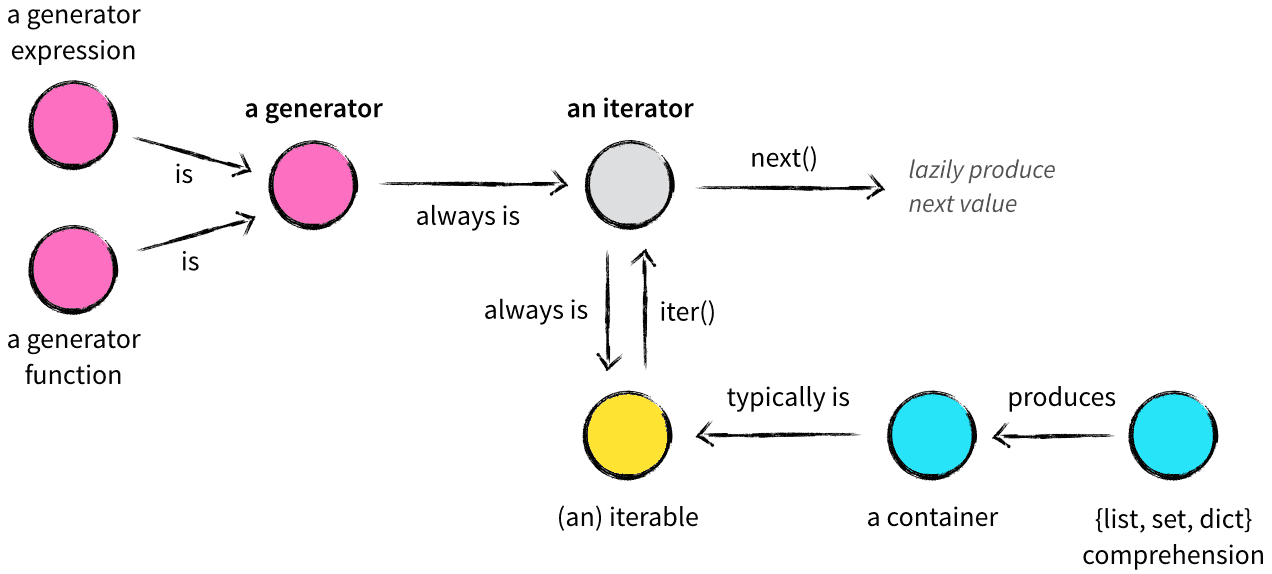
\includegraphics[width=0.9\linewidth]{relationships.png}\break
		{\tiny Quelle: \url{http://nvie.com/img/relationships.png}}
	\end{figure}
\end{frame}
\begin{frame}[fragile]{Generator-Expressions}
	\begin{itemize}
		\item Für einfache Iteratoren
		\item Gut für Iteratoren über vorhandene Daten
		\item Kann jedoch keine inneren Zustände haben 
	\end{itemize}
	\begin{grammatik}
		\begin{python}[numbers=none]
	gen_express = "(" comprehension ")"
		\end{python}
		\end{grammatik}
	\begin{example}
		\begin{python}[numbers=none]
°>>>° a = iter( [ x for x in range(10) ] )
°>>>° b = ( x  for x in range(10) )
°>>>° all( x == y for x, y in zip(a,b) )
True
		\end{python}
	\end{example}

\end{frame}
\begin{frame}[fragile, allowframebreaks]{Generator-Funktionen}
	\begin{itemize}
		\item Sehen Funktionen sehr ähnlich
		\item Benutzen das Keyword \emph{yield}
		\item Können innere Zustände haben
	\end{itemize}
	\begin{syntax}
		\begin{python}[numbers=none]
def name(*args, **kwargs):
	...
	yield x
	...
	
gen = name(*args, **kwargs)
		\end{python}
	\end{syntax}
\framebreak

\begin{example}
	\begin{python}[numbers=none]
°>>>° def fib():
§. . .§	  old, current = 0, 1
§. . .§	  while True
§. . .§	      old, current = current, current + old
§. . .§	      yield old

°>>>° f = fib()
°>>>° [ next(f) for i in range(10) ]
[1, 1, 2, 3, 5, 8, 13, 21, 34, 55]
	\end{python}
\end{example}
\framebreak

\begin{itemize}
	\item Der Generator arbeitet erst wenn \emph{next()} aufgerufen wird
	\item Es wird bis zum nächsten \emph{yield} ausgeführt, dann mit aktuellen Zustand pausiert
	\item Da immer nur ein Element berechnet und ausgegeben wird, sehr effizient
	\item Zusätzliche Methoden
	\begin{itemize}
		\item \textbf{send(value)} aktuelles \emph{yield} nimmt \emph{value} an
		\item \textbf{throw(exception)} wirft \emph{exception} an der Stelle von \emph{yield} 
		\item \textbf{close()} schließt Generator (wirft \emph{GeneratorExit})
	\end{itemize}
	\item Mit \emph{return} kann der Generator immer beendet werden
\end{itemize}

\framebreak

\begin{itemize}
	\item Generatoren eignen sich als Iterator in einer Klasse  
\end{itemize}
	\begin{exampleblock}~
	\begin{python}[numbers=none]
...
def __iter__(self):
	...
	yield x
	\end{python}
	\end{exampleblock}
\begin{itemize}
	\item Generatoren sind meistens schneller und speichereffizienter
	\item Iteratoren sind flexibler, als z.B. Listen
\end{itemize}
\end{frame}

\section{Dekorateure}
\begin{frame}[fragile, allowframebreaks]{Funktionen höherer Ordnung}
\begin{itemize}
	\item Alles in Python ist ein Objekt, auch Funktionen und Klassen
	\item Objekte kann man als Funktionsargument übergeben
	 
\end{itemize}
\begin{exampleblock}~
	\begin{python}[numbers=none]
def say_hi():
	return "hi"
	
def make_louder( f ):
	return f().upper()
	
shout_hi = make_louder(say_hi)
say_hi()	# "hi"
shout_hi()	# "HI"
	\end{python}
\end{exampleblock}

\framebreak

\begin{itemize}
	\item Ebenso können Funktionen von Funktionen zurückgegeben werden
\end{itemize}
\begin{exampleblock}~
	\begin{python}[numbers=none]
def first_n_squares( n : int ):
	def print_squares():
		print([i*i for i in range(1,n+1])
	return print_squares
	
first5 = first_n_squares(5)
first5() # [1, 4, 9, 16, 25]
	\end{python}
\end{exampleblock}
\end{frame}
\begin{frame}[fragile, allowframebreaks]{Decorator}
\begin{itemize}
	\item Dekorateure erwarten eine Funktion als Argument und geben eine Funktion zurück
	\item Um eine Funktion zu dekorieren schreibt man \emph{\bfseries @dec} in die Zeile über der Definition
	\item Diese Syntax ist gleichbedeutend mit \emph{f = dec(f)}
\end{itemize}
\framebreak
\begin{exampleblock}~
	\begin{python}[numbers=none]
def make_louder( f ):
	def wrapper(*args):
		print("In the Wrapper")
		result = f(*args)
		return result.upper()
	return wrapper

§@make_louder§
def say_hi():
	return "hi"

say_hi() 	# Prints "In the Wrapper"
			# Returns "HI"
	\end{python}
\end{exampleblock}
\end{frame}
\begin{frame}[fragile, allowframebreaks]{Nützliche Decorators}

\begin{example}[wraps, total\_ordering]
	\begin{python}[numbers=none]
from functools import wraps, total_ordering
def mydec(f):
	§@wraps§(f)
	def wrapper(*args, **kwargs): ...
	return wrapper
	
§@total_ordering§
class Human:
	def __eq__(self, other): ...
	def __gt__(self, other): ...
	\end{python}
\end{example}
\framebreak
	\begin{example}[contexmanager]
		\begin{python}[numbers=none]
from contextlib import contextmanager
§@contextmanager§
def get_score(path):
	scorefile = ...
	yield scorefile
	scorefile.close()
	
with get_score() ³as³ scores:
	scores.add( entry )
		\end{python}
	\end{example}
\framebreak
\begin{example}[lru\_cache]
\begin{python}[numbers=none]
from functools import lru_cache
§@lru_cache§(maxsize=2)
def fib(n):
	if n <= 1:
		return n
	return fib(n-2) + fib(n-1)
	\end{python}
\end{example}

\end{frame}
\appendix
\section<presentation>*{\appendixname}
\subsection<presentation>*{Quellen und weiterführende Informationen}

\begin{frame}[allowframebreaks]
  \frametitle<presentation>{Quellen und weiterführende Informationen}
    
  \begin{thebibliography}{10}
    
  \setbeamertemplate{bibliography item}[online]
  \bibitem{ABC}
	Handout und Beispiele als Jupyter-Notebooks
	\newblock {\scriptsize \url{https://mybinder.org/v2/gh/janDigeser/PythonSeminar/master}}
\medskip
\hrule
  \bibitem{ABC}
    Abstract Base Class Documentation
    \newblock {\scriptsize \url{https://docs.python.org/3/library/abc.html}}
    
  \bibitem{Lambda}
    Lamdba Funktionen und Beispiele
    \newblock {\scriptsize \url{https://www.python-kurs.eu/lambda.php}}
  
  \bibitem{ItvsGen}
	Iteratoren und Generatoren Unterschiede
	\newblock {\scriptsize \url{https://nvie.com/posts/iterators-vs-generators/}}
	
  \bibitem{yield}
	Dokumentation zum yield-Statement
	\newblock {\scriptsize \url{https://docs.python.org/3/reference/expressions.html\#yieldexpr}}
	
  \bibitem{PEP}
  	PEP über Generatoren
  	\newblock {\scriptsize \url{https://www.python.org/dev/peps/pep-0342/}}
    	
  \bibitem{Dec}
    Schnelle Einführung für Dekorateure
    \newblock {\scriptsize \url{http://jfine-python-classes.readthedocs.io/en/latest/decorators.html}}
    
  \bibitem{Dec2}
    Weiterführendes zu Dekorateure
    \newblock {\scriptsize \url{https://www.artima.com/weblogs/viewpost.jsp?thread=240808}
    \url{https://www.artima.com/weblogs/viewpost.jsp?thread=240845}}
    
  \end{thebibliography}
\end{frame}

\end{document}


